\subsection{Networking}\label{subsec:networking}

The \textbf{Networking} component is built on top of the \textit{Netty 5}\footnote{https://netty.io} networking framework.
It provides common abstractions used by both the API and the Gossip component.
Namely, it handles packet encoding and decoding, and connection establishment.

Packet serialization and deserialization can be implemented by conforming to the \ttt{OutboundPacket} or
\ttt{InboundPacket} interfaces (defining a respective \ttt{InboundPacketHandler}, respectively).
The set of supported packets can then be built using \ttt{ProtocolDescription} by supplying the packet
implementations and their corresponding packet ids.

Together with an \ttt{EventLoopGroup} instance, \ttt{ProtocolDescription}s can be used to instantiate
a \ttt{TCPClient} or \ttt{TCPServer} to bind the respective TCP socket.
\ttt{EventLoopGroup}\footnote{https://netty.io/4.1/api/io/netty/channel/EventLoopGroup.html}
is a concept provided by Netty, which manages a thread pool to handle incoming connections and
serialization of traffic asynchronously.

\subsubsection{Common Packet Format}

The \ttt{ConnectionInitializer} (automatically set up within the \ttt{TCPClient} or the \ttt{TCPServer})
constructs the channel pipeline for each connection.
The resulting channel pipeline is depicted in \autoref{fig:channel-pipeline}.
Incoming traffic passes through the \ttt{LengthFieldBasedFrameDecoder}\footnote{Provided by Netty: https://netty.io/4.1/api/io/netty/handler/codec/LengthFieldBasedFrameDecoder.html}
(parsing the \textit{size} field) and the \ttt{PacketDecoder} (parsing the \textit{packet id}, assembling the typed packet instances)
to the \ttt{InboundHandler}, calling the corresponding user code to handle the packet.
Outbound traffic passes the \ttt{PacketEncoder} (serializing the packet contents and writing the \textit{packet id})
and the \ttt{LengthFieldPrepender} (writing the \textit{size} field).

The illustrated channel pipeline results in the general packet header depicted in \autoref{fig:basic-packet-layout}.
The \textit{size} field is an unsigned 16-bit integer, resulting in a maximum packet size of
65535 bytes (including the header size).

\begin{figure*}[h!]
    \centering
    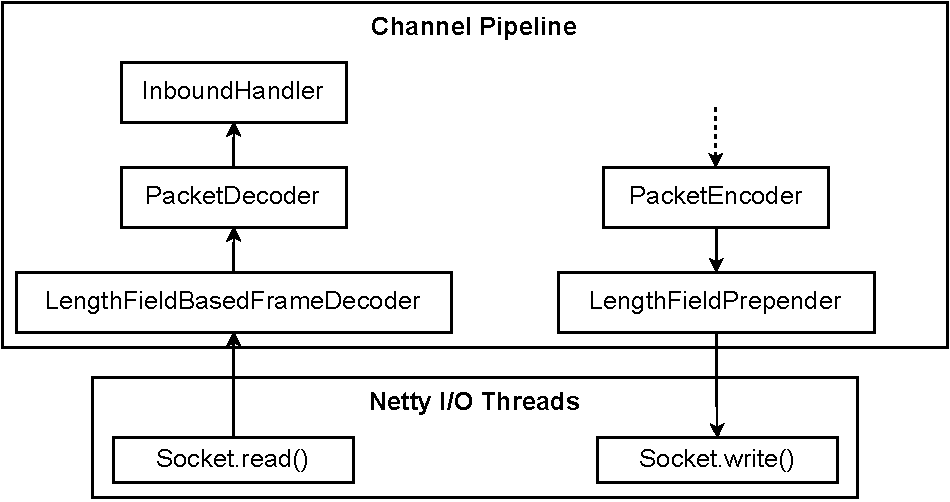
\includegraphics[width=1\linewidth, angle=0]{images/ChannelPipeline}
    \caption{Diagram of the Channel Pipeline of a open connection.}
    \label{fig:channel-pipeline}
\end{figure*}

\begin{figure}
    \centering
    \begin{bytefield}{32}
        \bitheader{0,7-8,15-16,23-24,30-31} \\
        \begin{rightwordgroup}{Packet \\  Header}
            \bitbox{16}{size} & \bitbox{16}{\texttt{packet Id}}
        \end{rightwordgroup} \\
        \begin{rightwordgroup}{Packet \\ Payload}
            \wordbox[tlr]{1}{} \\
            \skippedwords \\
            \wordbox[lrb]{1}{}
        \end{rightwordgroup}
    \end{bytefield}
    \caption{Packet header layout used within all packet types.}
    \label{fig:basic-packet-layout}
\end{figure}
